\section{Input-output systems estimation methods summary}

Consider a generic nonlinear dynamic system:
\begin{figure}[H]
    \centering
    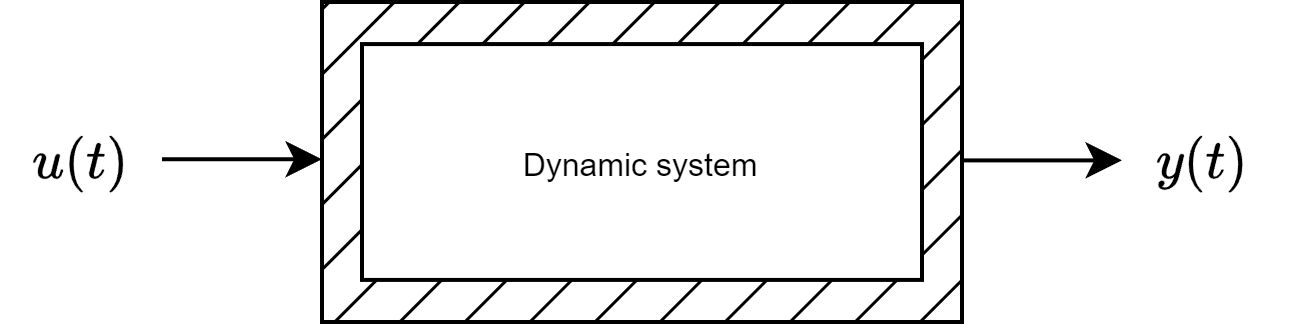
\includegraphics[width=0.6\linewidth]{images/sys1.png}
\end{figure}
In general, the process involves:
\begin{itemize}
    \item Collecting a dataset for training or model construction, which can be a natural collection or a designed experiment.
    \item Choosing a model framework (linear static, linear dynamic, nonlinear static, nonlinear dynamic) and the type of modeling (gray-box or black-box).
    \item Selecting an estimation approach (constructive 4SID, parametric optimization, and filtering).
\end{itemize}

\subsection{Black-box versus white-box}
The choice between black-box and white-box modeling depends on the context.

The black-box approach, utilized by Machine Learning, leverages all available data. 
It offers versatility, flexibility, and fully exploits data without requiring specific knowledge of the system's physics. 
However, incorporating physical knowledge can enhance the effectiveness of the black-box approach.
The popularity of black-box modeling has surged due to:
\begin{itemize}
    \item The ease of collecting and storing digital data.
    \item Advances in computational power.
\end{itemize}
However, white-box modeling remains valuable for system designers, providing deeper insights into the system's inner workings.